% Kapitel 3

\chapter{Data Efficiency via Model-Driven Preprocessing}
\label{chap:model-driven-preprocessing}

% todo: maybe some sort of introduction what we will show
% first, how preprocessing can achieve data efficiency
% next, the limitations of traditional preprocessing
% next, using neural networks to find preprocessing parameters

In this chapter, we will propose another way of achieving data efficiency in neural network-based medical image segmentation. We will first describe yet another way to view neural networks --- as algorithms to find a linearly separable transformation of an input space. To simplify, let us focus on a 2-class classification problem, with a dataset ${(X_i, Y_i)}, X_i \in \mathbb{R}^2, Y_i \in \{0, 1\}$. All of our input vectors $X_i$ come from an input space $\mathcal{X}$. The neural network is tasked with finding a decision boundary that splits the input space into two sides, one labeled 0 and the other labeled 2. For complex problems, this decision boundary is not linear in the input space. For instance, we can imagine a dataset where points belonging to class 0 are clustered around $(0, 0)$, while points belonging to class 1 are distributed along a circle with radius 2 with additive Gaussian noise, as is shown in \figref{fig:input-space-transform}(left). In the input space, the optimal decision boundary is circular, and therefore the input space cannot be linearly separated in its current form. Instead, a neural network learns a transformation $\mathcal{X} \rightarrow \mathcal{X'}$ such that a hyperplane can be drawn in $X'$ to optimally separate points belonging to classes 0 and 1. This is illustrated in \figref{fig:input-space-transform}(right). 

	\begin{figure}[h]
		\centering
		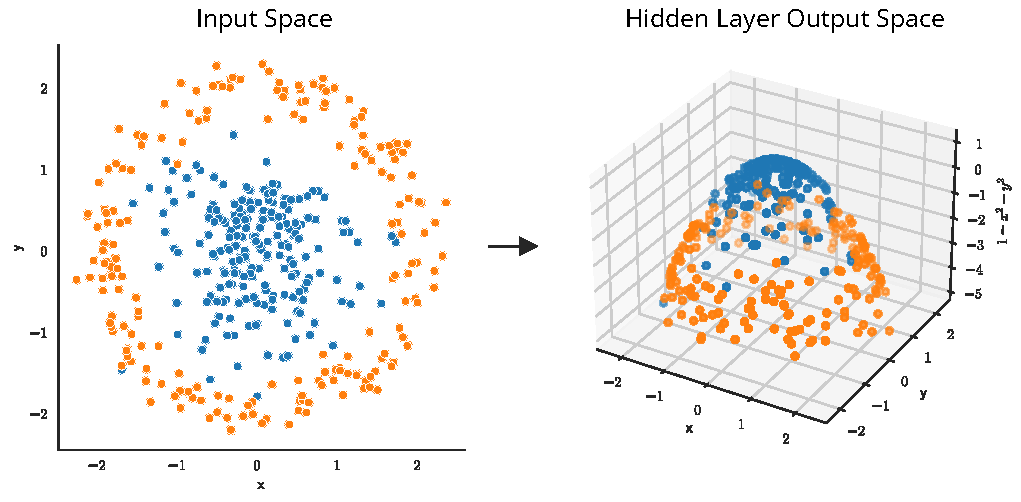
\includegraphics[width=0.65\linewidth]{images/4/nn_trans_dataset}
		\caption{An example of how a 2-class classification neural network bends an input space (left) such that it is linearly separable with a hyperplane.}
		\label{fig:input-space-transform}
	\end{figure}

To do this, the network needs sufficient parameters --- more parameters allow for more complex transformations. Without enough parameters, no hyperplane in the transformed space can separate the two points well, leading to underfitting. To approach correctly approximating a circular decision boundary, the network needs at least three neurons in its hidden layer. We exemplify this in \figref{fig:circ-datataset-neurons}.

	\begin{figure}[h]
		\centering
		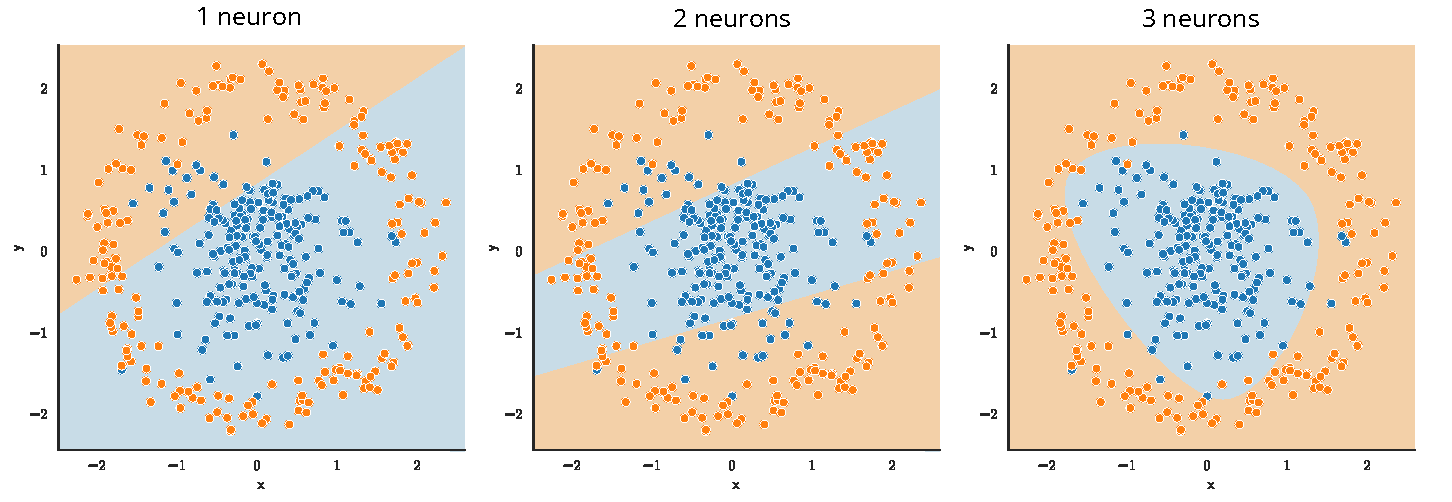
\includegraphics[width=\linewidth]{images/4/circular_dataset_neurons}
		\caption{The decision boundary (shown as the background color) according to a fully connected neural network with one hidden layer where the hidden layer has one, two, or three neurons.}
		\label{fig:circ-datataset-neurons}
	\end{figure}

Therefore, we will focus on finding transformations of the data such that the problem becomes easier. To illustrate why this is effective, we will present yet another view of neural networks. Let there be some neural network that we are using to determine whether a given image region $I(x, y)$ belongs to class ``0'' or ``1''. All possible image regions $I(x, y)$ come from a $d$-dimensional space called the input space where $d$ is the number of pixels in the region, multiplied by the number of channels in each pixel. Through optimization, the neural network iteratively finds a transformation of the input space such that this space can be linearly separated by a $d$-dimensional hyperplane into two classes. This is illustrated in \figref{fig:input-space-transform}.

The goal of data efficiency is to find a decision boundary given fewer data samples. As discussed in the previous chapter, this necessitates reducing the function class space we are searching over, or in other words, reducing the number of neural network parameters. In this and the following chapters, we will focus on finding ways to pre-transform the data into some intermediary form $\mathcal{X}_{pre}$ that is more separable than the original input space $\mathcal{X}$. This allows networks with fewer parameters, as $\mathcal{X}_{pre}$ is closer to $X'$, and thus the network has to search a smaller space to find $X'$. We will call this transformation $\mathcal{T}$.

An commonly used example of $\mathcal{T}$ is the polar transform, wherein an input vector $X_i = [x_0, x_1]$ is transformed into a vector $\mathcal{T}(X_i) = [\theta, r]$ as:

\begin{equation}
    \begin{aligned}
	r =& \sqrt{x_0^2 + x_1^2},\\
	\theta =& atan2(x_1, x_0).
    \end{aligned}
\end{equation}

The polar transforms turns a circular decision boundary into a linear one, allowing linear separability of our example dataset even given only one neuron in the neural network, as can be seen in \figref{fig:polar_dataset_neurons}

	\begin{figure}[h]
		\centering
		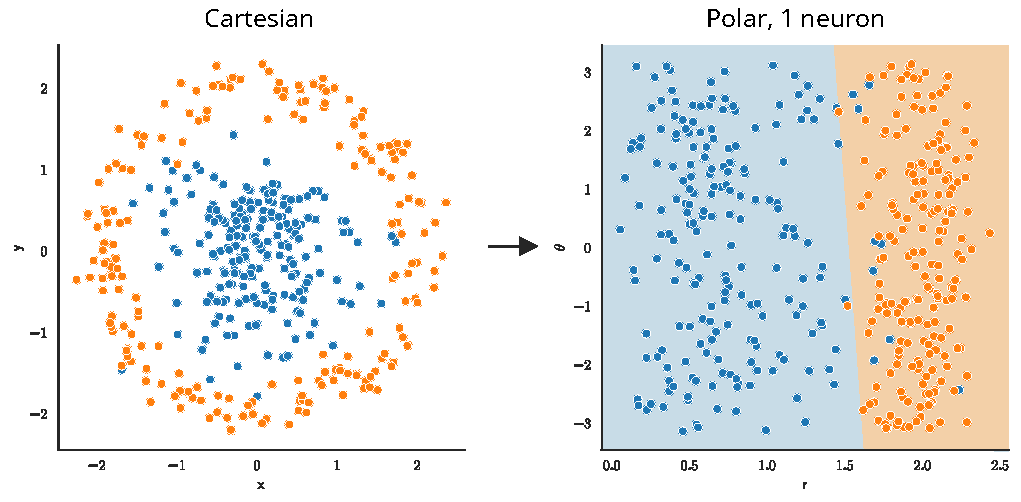
\includegraphics[width=0.65\linewidth]{images/4/polar_dataset_neurons}
		\caption{An example circular dataset transformed using the polar transform. The background color shows the decision boundary of a fully connected network with one hidden layer with a single neuron.}
		\label{fig:polar_dataset_neurons}
	\end{figure}

Here, we have shown how using the polar transform already transforms the input space into a linearly separable form. The network effectively only needs to search the space of lines to find one that optimally separates the two classes.

% explain transformation parameters, origin is (0, 0), but doesn't have to be
% explain how we need to predict the origin to produce useful transformation, we can use a neural network for this

% tie in with regularization somehow

% from understanding ml ben david:
% The transformation from the real world object “papaya” into the scalar representing its softness or its color is called a feature function or a feature for short; namely, any measurement of the real world object can be regarded as a feature. If X is a subset of a vector space, each x ∈ X is sometimes referred to as a feature vector. It is important to understand that the way we encode real world objects as an instance space X is by itself prior knowledge about the problem.
% Furthermore, even when we already have an instance space X which is rep- resented as a subset of a vector space, we might still want to change it into a different representation and apply a hypothesis class on top of it. That is, we may define a hypothesis class on X by composing some class H on top of a feature function which maps X into some other vector space X′.

% maybe thresholding can be feature selection

% add sections about example transformations that are useful, with prior knowledge?



% maybe https://colah.github.io/posts/2014-03-NN-Manifolds-Topology/
% or maybe look for polar in goodfellow deep learning

\todo{some sort of introduction}

\section{Motivation}

As mentioned in the previous chapter, aside from getting new data, the easiest way to reduce the estimation error is by limiting the size of the function class our model optimizes. In a traditional machine learning approach, this would be done by hand-selecting a class of functions with a lower number of parameters and then training the model. In deep learning, however, this approach is usually replaced with \textbf{regularization}, where the parameters themselves are manipulated to simplify the model.\footnote{Often, any method of reducing the estimation error of the model is broadly termed as regularization.} Instead of selecting the number of parameters, we can penalize the network for the complexity and size of the parameters. In other words, the loss function between a predicted model output $y_{pred}$ and a ground-truth label $y$ has the form:

\begin{equation}
	L(\theta; y_{pred}, y) = L_{seg}(\theta; y_{pred}, y) + \alpha\Omega(\theta)
\end{equation}

where $L_{seg}$ is the segmentation loss function while $\Omega(\theta)$ is a parameter norm penalty, i.e. a measure of the complexity of the model \cite{goodfellowDeepLearning2016}. As we increase $\alpha$, the strength of the regularization increases and the loss is more impacted by the complexity of the model. As the network is being trained, it will seek to both reduce $\Omega(\theta)$ as well as $L_{seg}$, leading to a more constrained model.

A commonly used parameter norm penalty is the $L^2$ regularization, also known as \textbf{weight decay} in deep learning contexts. Assuming $\theta$ consists of a set of weights $w, \lvert w \rvert = n$ and biases $b$, the $L^2$ norm is defined as $\Omega(w) = \frac{1}{2}\sqrt{(w_1^2 + w_2^2 + \cdots + w_n^2)}$. In other words, the network is exponentially penalized for moving weights away from zero. This regularisation, in effect, forces the network to use fewer parameters.

% TODO: Feature transformation from ML book?
% TODO: A proxy measurement of segmentation complexity, how many parameters to model a decision boundary?

Thus, a deep learning network can learn to use fewer parameters without necessarily changing the architecture of the network itself. However, what remains unsolved is how to transform the data such that the network can solve the problem with fewer parameters.

\section{Model-driven Preprocessing to Simplify Segmentation Problems}

We will illustrate this using an example of segmenting epicardial fat on CT scans. Epicardial fat has a complex and sparse distribution between the heart wall and the pericardium, a thin fibrous protective sac around the heart, as can be seen in \todo{figure}. This is a hard segmentation problem, as the complex shape requires a large amount of parameters to model. 

We can simplify the segmentation problem with two transformations. First, we can use thresholding to remove irrelevant pixels from the image. In CT scans, each tissue falls within a known range of intensity values. Empirically, it has been determined that epicardial fat falls roughly in the range of $[-190, -30]$ HU. By removing all pixels outside of this range, we reduce the amount of information in the image without removing any epicardial fat pixels. This allows the model to more easily segment the image, as it does not need to learn to remove these irrelevant pixels itself.

Next, we can further simplify the segmentation problem by segmenting a simpler shape. By definition, epicardial fat is located within the pericardium, which has a smooth elliptical shape around the heart. Since we have already thresholded the image, all pixels within the pericardium are epicardial fat. Thus, the problem of segmenting epicardial fat can be reduced to segmenting the pericardium. Given its smooth and simple shape, the model requires much fewer parameters to model the pericardium compared to the complex epicardial fat distribution. When formulated this way, the problem of segmenting epicardial fat can even be solved by using much simpler methods such as ellipse fitting instead of neural networks \todo{cite}.

This example demonstrates an approach of preprocessing images guided by domain knowledge to allow segmentation with much fewer parameters. However, this approach suffers from a key problem. The preprocessing parameters, such as the thresholds for epicardial fat, need to be selected ahead of time and kept static. However, the exact Houndsfield range of epicardial fat varies from patient to patient \todo{cite}. 

\subsection{Estimating Preprocessing Parameters Using Neural Networks}

To overcome this problem, we propose an approach where the transformation parameters are determined by a neural network based on the input image. In the example of epicardial fat segmentation, the parameters would be the threshold values for the epicardial fat. Formally, we can express this approach as segmenting a transformed image:

\begin{equation}
	M(I) = F_{seg}(\mathcal{T}(\phi)(I); \theta_{seg}),
\end{equation}

where $M(I)$ is the resulting segmentation mask for image $I$, $F_{seg}$ is a segmentation neural network with parameters $\theta_{seg}$ and $\mathcal{T}$ is a functional giving a transformation functions for a given set of transformation parameters $\phi$. The transformation can be any transformation function including affine transformations, deformation fields as well as thresholding, as in the above example. The parameters $\phi$ are estimated with a second neural network:

\begin{equation}
	\phi(I) = F_{\mathcal{T}}(I; \theta_{\mathcal{T}}),
\end{equation}

where $F_{\mathcal{T}}$ is a neural network with parameters $\theta_{\mathcal{T}}$ trained to estimate the correct parameters for $\mathcal{T}$ given an image $I$.

The core idea is that $\mathcal{T}$ will simplify the segmentation problem such that a regularized segmentation network $F_{seg}$ will be able to perform the segmentation using fewer parameters. To achieve this, both $F_{\theta}$ and $F_{seg}$ need to be trained using specific training methods, as we will describe in the next section.

% TODO: benefits: transfer learning, weakly supervised, simpler networks instead of one large one

\section{Preprocessing With the Polar Transform Using Centerpoint Prediction}

Images are most commonly viewed in Cartesian coordinates, where the pixels are arranged along the x- and y-axes. The polar coordinate system has two axes: (1) the radial coordinate $
\rho$, which is the distance 
of a point from the origin of the polar transformation; and (2) the angular coordinate $\phi$, which is the angle 
between the point and the reference direction. In other words, the x-axis of the polar image represents the 
distance from an origin, while the y-axis represents the rotation around the origin. This makes polar coordinates 
invariant to rotation.

Our intuition is that polar transformations can be especially beneficial to segmenting images where an 
elliptical border must be found on the image. Consider a contrived example of predicting a 
circular decision boundary on a single-channel image with a linear model. A circular decision boundary 
must be modeled by a function of at least four dimensions. When transformed to 
polar coordinates, a perfect circle in Cartesian coordinates becomes a straight line, as shown in 
\figref{fig:polar-coords}. This linear decision boundary can be modeled with a simpler linear function 
in two dimensions. The image in polar coordinates would require a less complex model to predict a 
border. It is possible that, even for more complex examples, the polar transform of an image of a roughly 
elliptical object reduces the required segmentation model complexity, as shown visually in 
\figref{fig:polar-lesion}. Furthermore, by transforming an image to polar coordinates using a polar origin 
that is the center of the object, we fix the location and standardize border distances in each training 
example. The model can then learn the distance of the border from the origin at each angle around the 
origin, without having to learn to localize the object.

	\begin{figure}[h]
		\centering
		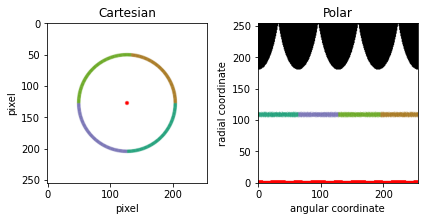
\includegraphics[width=0.6\linewidth]{images/4/polar-transform}
		\caption{An example of a polar transformation.}
		\label{fig:polar-coords}
	\end{figure}


	\begin{figure}[h]
		\centering
		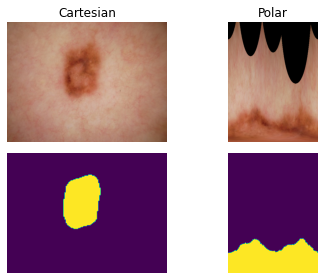
\includegraphics[width=0.4\linewidth]{images/4/to_polar}
		\caption{An example image and label from the lesion dataset and their corresponding polar transformation.}
		\label{fig:polar-lesion}
	\end{figure}

To obtain a polar 
transformation, the angle and magnitude of each pixel $(x, y)$ of the original image are 
calculated using \eqref{eq:magang}:

  \begin{equation}
    \begin{aligned}
      magnitude(x, y) &= \sqrt{x^2 + y^2} , \\ 
      angle(x, y) &= atan2(y, x) [ \cdot 180 / \pi ]
    \end{aligned}
    \label{eq:magang}
  \end{equation}

Where $atan2$ is the 2-argument arctangent function.

Given a polar origin $(c_x, c_y)$ of a Cartesian image $I(x, y)$ of resolution $H \times W$, we obtain each point $(\rho, \phi)$ of the polar transformation $I'(\rho, \phi)$ using 
\eqref{eq:polar-transform}.

  \begin{equation}
    \begin{aligned}
      \rho &= \frac{H}{2 \Pi} \cdot angle(x - c_x, y - c_y) \\
      \phi &= \frac{W}{\sqrt{(W / 2)^2 + (H / 2)^2}} \cdot magnitude(x - c_x, y - c_y)
    \end{aligned}
    \label{eq:polar-transform}
  \end{equation}

\todo{formulate problem and introduce using the above framework}

In this chapter, we propose a general way to improve neural network segmentation data efficiency and performance 
on medical imaging segmentation tasks where the goal is to segment roughly 
elliptically distributed objects.

We propose and explore ways to train neural networks for biomedical image segmentation on polar transformations of images. The polar transformation transforms an image from Cartesian coordinates into a new coordinate system where the two
axes are the rotation around an origin and radius from that origin. When the regions to be segmented are elliptical in shape or distribution, this transformation results in a reduction of dimensionality, allowing convergence in fewer epochs and good performance even in models with a low number of parameters. 

Experimentally, we observed that selecting
a correct polar origin is one of the key parameters that determine segmentation performance. Therefore, we propose two 
different approaches of selecting an optimal polar origin: (1)
estimation via a segmentation neural network trained on non-polar images and (2) estimation via a neural network trained
to predict heatmaps.
Our method is evaluated on 
the tasks of polyp segmentation, liver segmentation, skin 
lesion segmentation, and epicardial adipose tissue (EAT) segmentation.
The proposed methods can be used as a pre-processing step for 
existing neural network architectures, so we evaluate the methods using
common neural network architectures for medical image segmentation including U-Net 
\cite{ronnebergerUNetConvolutionalNetworks2015}, U-Net++ 
\cite{zhou2019unetplusplus} with a ResNet \cite{heDeepResidualLearning2016} encoder, and DeepLabV3+ \cite{chenEncoderDecoderAtrousSeparable2018} with a ResNet \cite{heDeepResidualLearning2016} encoder.

Evaluation of our approach as a pre-processing step shows that it improves segmentation performance across different datasets and neural network architectures while making the networks more robust to small dataset sample sizes.

    \subsection{Previous work using the polar transform for medical image processing}
    
Several image segmentation methods were proposed that utilize polar coordinates. 
\citet{liuDDNetCartesianpolarDualdomain2019a} proposed an approach they
call Cartesian-polar dual-domain network (DDNet) to perform optic disc and cup segmentation
in retinal fundus images. The neural network contains two encoding branches, one for a Cartesian input image and another for the polar transformation of the same input image. The predictions are fused into a single feature vector which is then decoded into a final segmentation.
\citet{salehinejadImageAugmentationUsing2018} used the polar transformation as a way to 
augment
training data by transforming each input image into multiple polar images at various polar
origins, thus increasing the number of training data.
\citet{kimCyCNNRotationInvariant2020a} proposed a convolutional neural network layer for 
images in polar 
coordinates to achieve rotational invariance. Their cylindrical convolution layer uses cylindrically sliding windows to perform a convolution.
\citet{kimCNNBasedUGS2018} proposed a user-guided segmentation method where an expert 
selects the
point used as the polar origin. The transformed image is then
segmented using a convolutional neural network (CNN). 
\citet{estevesPolarTransformerNetworks2018a} proposed a polar transformer network for image 
classification. Note that "transformer network" here refers to spatial transformer networks 
\cite{jaderbergSpatialTransformerNetworks2016} and not attention-based networks commonly called 
transformers.
The network 
consist of a polar origin predictor and a neural network that predicts a heatmap. The centroid of the heatmap is then used as the origin for a polar transformation of the input image. The polar image is classified using a CNN. This approach is most similar to our proposed method, 
however, their approach focuses on image classification, not segmentation. Additionally, our approach differs in the ways the ground truth data is prepared, the used neural network architectures, as well as other details.

While there are proposed methods that combine polar transformation with neural networks, most of them solve classification tasks. Some medical image segmentation methods use the polar transformation as a preprocessing step, however, the way they obtain the origin of the polar transformation is usually based on heuristics. To our knowledge, there is currently no work that explores using the polar transformation with a dynamic polar origin as a preprocessing step for semantic segmentation in a variety of medical image datasets.

  \subsection{Methodology}
  
All of the proposed methods rely on training a neural network model to segment polar images. To train on 
polar images, the input images need to be transformed using a polar origin which is near the center of 
the 
segmented object. The correct origin is not known ahead of time, so a prerequisite for predictions on polar
images is a method to determine the correct polar origin. We propose and 
evaluate two different methods for automatically obtaining the polar origin: (1)
estimation via a segmentation trained on non-polar images and (2) training a center-point predictor that predicts heatmaps from input images. 
This section describes these methods, as well as methods to train the 
final segmentation model on the polar images.
      
In each of our approaches, the final segmentation is done using a neural network trained on polar 
transformations of the input images. In the rest of this paper, we refer to this network as the polar 
network. In all of the described approaches, the polar transformation is not part of the network architecture itself, but happens as a preprocessing step for the polar network.
To transform each input image, the polar origin is determined as the center of mass of the 
ground truth label for that image. The center of mass of an image $I(x, y)$ is calculated by first 
calculating the spatial image moments matrix $M$, where the entry of the matrix at row $i$ and column $j$ is calculated using \eqref{eq:moments}.

  \begin{equation}
    M_{ij}= \sum _{x,y} I(x,y) \cdot x^i \cdot y^j
    \label{eq:moments}
  \end{equation}
  
The center of mass $(c_x, c_y)$ of the image can then be calculated using \eqref{eq:center-mass}.

  \begin{equation}
    \begin{aligned}
      c_x &= M_{10} / M_{00} \\
      c_y &= M_{01} / M_{00}
    \end{aligned}
    \label{eq:center-mass}
  \end{equation}

Finally, to increase the model's robustness to suboptimal center point predictions, we augment the 
calculated center for training images \cite{estevesPolarTransformerNetworks2018a}. Each training image has 
a 30\% chance of varying the center's x and y coordinates by a random value in the range $(-S \cdot 0.05, 
S \cdot 0.05)$, where $S$ is the smallest resolution of the image, i.e. $S = min(width, height)$.
 
    \subsection{Centerpoint prediction}
    
Once the polar network is trained, inference can be done by transforming an input image to polar 
coordinates. The polar network requires choosing a center that is close to the center of mass of the 
segmented object. Because a future input image is unlabeled, the correct center needs to be inferred from 
the image. We propose two ways to accomplish this, described in this section.

   \subsubsection{(A) Training the same neural network on cartesian and polar images}
   \label{retraining-approach}
   
Our first approach is training the same neural network on cartesian and polar images. A summary of this
approach is presented in \figref{fig:retraining-diagram}. With this approach, 
the inference is done by first feeding the original Cartesian input images into a neural 
network used for segmentation. We refer to this network as the Cartesian network.
For an input image, the polar origin is calculated as the center of mass of the Cartesian network's
prediction for that input image, using \eqref{eq:center-mass}.
This polar origin is used to transform the original input image to polar coordinates, and the transformed 
image is fed
to the polar network. The output of the polar network is transformed back to Cartesian coordinates
to obtain a final segmentation. We assume 
identical architectures for both the Cartesian and polar networks. This makes applying this
framework to existing architectures very straightforward, as it does not require designing new neural 
network architectures or specific hyperparameter optimization, and allows for using transfer learning to
initialize the networks.

	\begin{figure*}[h!]
		\centering
		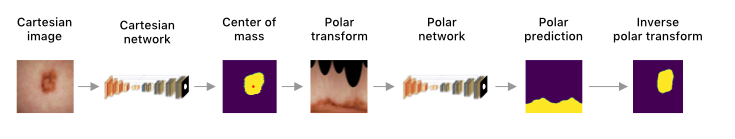
\includegraphics[width=\linewidth]{images/4/retraining-approach}
		\caption{A diagram of the approach of predicting polar origins from a Cartesian network. The first network performs an initial segmentation, which is then used to extract a polar origin for the polar transformation. The method does not rely on any specific neural network architure. The Polar and Cartesian network can be any neural network which takes an input image and produces a binary segmentation mask as output. The red point shows the extracted polar origin. The Polar network is trained on polar image transformations. The polar transformation is not part of the network itself, but happens as a preprocessing step for the Polar network.}
		\label{fig:retraining-diagram}
	\end{figure*}
	
    \subsubsection{(B) Training a centerpoint predictor}
    \label{centerpoint-approach}
    
In the second approach for determining the optimal polar origin, we train a model specifically tasked with predicting the correct
polar origin for each input 
image, which is then used to transform the input image. The approach is shown in \figref{fig:centerpoint-approach}. 
We do this by training a neural network based on the stacked hourglass architecture 
\cite{newellStackedHourglassNetworks2016} first used for human pose estimation. Instead of training a regressor network to
predict key points in an image, the stacked hourglass architecture uses a series of stacked encoder-decoder networks, where the output
of each stack is a heatmap centered on the key point to be predicted. The output of each stack is fed as input into the next stack, allowing 
successive refinement of the heatmap prediction. During training, the loss of each stack's output is averaged to produce the final loss, 
allowing deep supervision. The final prediction heatmap is the output of the last stack in the network. To predict the center point, 
we use 8 stacked hourglass blocks, which we empirically determined as the value providing the best results. The network receives images in Cartesian 
coordinates and predicts a heatmap of the image.

	\begin{figure*}[h]
		\centering
		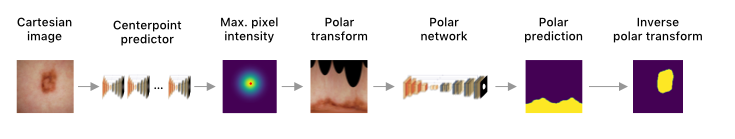
\includegraphics[width=\linewidth]{images/4/centerpoint-approach}
		\caption{A diagram of the approach of using a centerpoint prediction network. The first network can be any neural network which predicts a heatmap from an input image, which is then used to extract polar origin, shown as a red point. The Polar network can be any semantic segmentation neural network which produces a binary mask output from an input image. The Polar network is trained on polar image transformations. The polar transformation is not part of the network itself, but happens as a preprocessing step for the Polar network.}
		\label{fig:centerpoint-approach}
	\end{figure*}
 
The ground truth heatmaps were generated by calculating the center of mass of each ground truth label 
image using \eqref{eq:center-mass}. We then create the heatmap as an image with a 2D gaussian with the
mean on 
the center of mass on the image and a standard deviation of 8 pixels for all datasets except the liver, and 16 for the liver.
Example heatmaps are shown in 
\figref{fig:heatmap}. The optimal value for the standard deviation was determined empirically on the 
validation datasets. We found that the optimal value of the standard deviation is proportional to the size 
of the object.

	\begin{figure}[h]
		\centering
		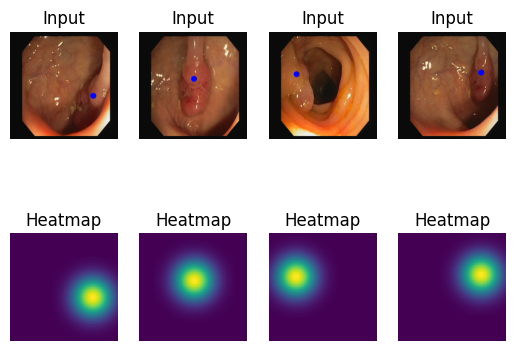
\includegraphics[width=0.8\linewidth]{images/4/heatmaps}
		\caption{Examples of heatmaps generated from the ground truth data. The heatmap is a gaussian centered on the center of mass of the ground-truth label, shown as a blue point on the input images.}
		\label{fig:heatmap}
	\end{figure}

Additionally, during training, we use augmentation to increase the number of training inputs. In 
particular, during training each input example the following random augmentations are applied:

\begin{itemize}
  \item A 50\% chance of a horizontal flip.
  \item A 30\% chance of a random combination of shifting up to 6.5\% of the image dimensions, scaling up 
    to 10\% and rotating up to 45$^{\circ}$.
  \item A 30\% chance for a grid distortion, details of which are described in \cite{info11020125}.
\end{itemize}

The center-point predictor outputs 8 separate heatmaps \cite{newellStackedHourglassNetworks2016}. We
calculate the predicted center as the coordinates of the pixel with the largest intensity in the heatmap
predicted by the final layer of the model. This predicted center is then used to transform the input
image to polar coordinates, and the transformed image is fed into the polar network to perform
the segmentation. Finally, the segmentation label is transformed back to Cartesian coordinates.
    
  \subsection{Experiments} \label{experiments}
  
To validate the generality of our approach, we trained a variety of neural network architectures on 
multiple medical imaging datasets. In particular, we trained three different neural network 
architectures: U-Net \cite{ronnebergerUNetConvolutionalNetworks2015}, U-Net++ 
\cite{zhouUNetNestedUNet2018a} with a ResNet encoder and DeepLabV3+ 
\cite{chenEncoderDecoderAtrousSeparable2018a} with a ResNet encoder. Notably, each dataset we use presents a problem wherein almost all examples a single roughly elliptical object needs to be segmented. 
For each dataset and network architecture combination, we train a Cartesian and polar network, and we then 
perform four different experiments: 

\begin{enumerate}
	\item{testing the Cartesian network using Cartesian images}
	\item{testing the polar network using the ground-truth polar origin}
	\item{testing the polar network using polar origins obtained from predictions of the Cartesian network, as outlined in \ref{retraining-approach}}
	\item{testing the polar network using polar origins from the center-point predictor, as outlined in \ref{centerpoint-approach}}.
\end{enumerate}

    \subsection{Datasets description}

We used four different datasets to train the network. In this section, we give an overview of each used dataset and how it was preprocessed. Note that for training the center-point predictor, the input images were resized to a resolution of $256 \times 256$, while the generated heatmaps were resized to $64 \times 64$ pixels. Otherwise, all preprocessing steps described here are applied to the center-point model datasets as well. Each dataset was normalized and zero-centered to better facilitate network convergence. 

	\begin{figure*}
	\subfloat[Polyp dataset]{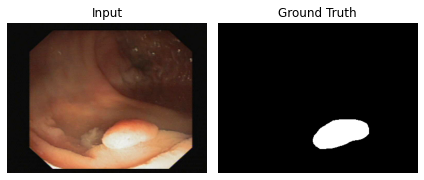
\includegraphics[width=0.49\columnwidth]{images/4/polyp_example}}
	\hfill
	\subfloat[Lesion dataset]{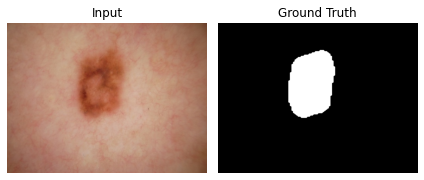
\includegraphics[width=0.49\columnwidth]{images/4/lesion_example}} \\
	\subfloat[Liver dataset]{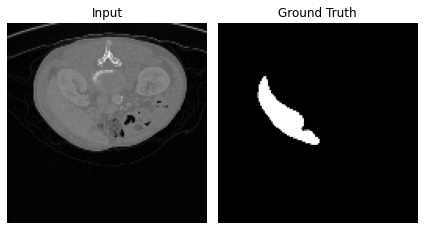
\includegraphics[width=0.49\columnwidth]{images/4/liver_example}}
	\hfill
	\subfloat[EAT dataset]{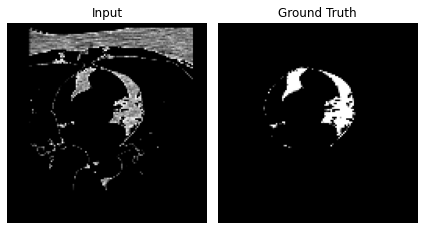
\includegraphics[width=0.49\columnwidth]{images/4/eat_example}} \\
	\caption{Example input images and ground-truth labels for each dataset used in our experiments.}
	\label{fig:datasets}
	\end{figure*}

      \subsubsection{Polyp dataset}

The CVC-ClinicDB dataset
\cite{bernalWMDOVAMapsAccurate2015} contains 612 RGB 
colonoscopy images with the resolution $288 \times 384$ 
with labeled polyps from MICCAI 2015. We normalize each image to a range of $[-0.5, 0.5]$. 
We use the original image resolution to train all networks except the 
centerpoint network. As is used in \cite{jhaDoubleUNetDeepConvolutional2020}, 
we use an 80\%, 10\% and 10\% 
split for training, validation and testing datasets, respectively. An example of the dataset is shown in \figref{fig:datasets}(a).

      \subsubsection{Liver dataset}

The second dataset we use is the LiTS dataset \cite{bilicLiverTumorSegmentation2019} from the Liver Tumor Segmentation Challenge from MICCAI 2017. The dataset contains 131 CT scans of patients with hepatocellular carcinoma, with the liver as well as tumor lesions labeled by experts. In our experiments, we disregard the lesion segmentation labels and treat the dataset as a binary liver segmentation problem. In addition, we removed all slices that did not contain a ground-truth liver segmentation label, resulting in a dataset of roughly 15,000 slices. Each axial slice is thresholded to a Hounsfield scale range of $[0, 200]$ HU that contains the liver. Next, the slices are normalized to a $[0, 1]$ range and zero-centered by subtracting the global intensity of all training slices (0.1). We then proceed to train the networks on each axial slice separately. We use 101 scans for training, 15 scans for validation, and the remaining 15 scans for testing. Example liver segmentation images are shown in \figref{fig:datasets}(c).

      \subsubsection{Lesion dataset}

The third dataset we use is the ISIC 2018 Lesion Boundary Segmentation dataset 
\cite{codellaSkinLesionAnalysis2018, tschandlHAM10000DatasetLarge2018} which contains 2,694 dermatoscopy 
images of skin lesions with expert labels of the lesions from various anatomic sites and several different 
institutions. We resize each image to a 
resolution of $384 \times 512$ and use a training, validation and test split of 80\%, 10\% and 10\%, 
respectively. This is consistent with \cite{jhaDoubleUNetDeepConvolutional2020}. Additionally, we normalize 
each image to a range of $[-0.5, 0.5]$. An example of a lesion 
input image and its corresponding label is shown in \figref{fig:datasets}(b).
	
      \subsubsection{EAT dataset}

Finally, we also train on a dataset of labeled EAT regions from 20 patients' cardiac CT scans from 
the Cardiac Fat Database \cite{rodriguesNovelApproachAutomated2016}. The dataset has three classes labeled: 
the pericardium, EAT, and pericardial adipose tissue. We disregard all original labels except EAT and treat the dataset as a binary EAT segmentation dataset. The dataset is 
first split into training (10 patients), validation (5 patients), and test (5 patients) datasets. In the 
original dataset, 
each slice is thresholded to the adipose tissue range of $[-200, -30]$ HU and registered so that anatomical 
structures have the same locations. In addition to these original pre-processing steps, we normalize each 
slice to a $[0, 1]$ range and zero-center 
the dataset by subtracting a global mean intensity of the training set (0.1). We then train on 
each CT slice separately. An input image of the EAT dataset and its corresponding label is shown in 
\figref{fig:datasets}(d).

    \subsection{Implementation details}

We use the OpenCV linear polar transformation implementation.
Each model is implemented and trained using PyTorch 1.7.1 on an NVIDIA GeForce RTX 3080 GPU. For all 
networks, we use the Adam optimizer with a learning rate of $10^{-3}$. A batch size of 8 was used for all 
networks except the center-point model, where a batch size of 6 was used for the lesion and liver datasets, 
and 8 for all remaining datasets. We trained all models up to a maximum of 200 epochs and used checkpoints 
after each epoch to store the model with the best validation loss. We modify the Dice coefficient to act as a loss function as shown in (\ref{eq:dice-loss}).

  \begin{equation}
    \textit{DSC}_{loss} = 1 - \frac {2\lvert X\cap Y\rvert + \lambda}{\lvert X\rvert + \lvert Y\rvert + \lambda}
    \label{eq:dice-loss}
  \end{equation}
  
Where $X$ and $Y$ are the input and predicted images, respectively, and $\lambda$ is a smoothing parameter set to 1 in our experiments. 
This loss function is used to train all models except the center-point model.

The centerpoint model outputs eight heatmaps \cite{newellStackedHourglassNetworks2016}. 
We use a loss function that is the mean of the mean squared errors between each of the heatmaps and the ground truth heatmap.
The code used for all experiments is available at \url{github.com/marinbenc/medical-polar-training}.

  \subsection{Results}

% ---------- RESULT  TABLES ---------- %

\begin{table}
\centering
\def\arraystretch{1.25}
\begin{tabular}{l l c c c c} 
 \hline \\ [-2ex]

 \multicolumn{6}{c}{\textbf{Polyp Segmentation}}\\[1ex]
 \hline
 Architecture & Method & DSC & mIoU & Prec. & Rec. \\ 
 \hline \\ [-1.5ex]
 
 \multirow{4}{7em}{{U-Net}}
& Cartesian & 0.8315 & 0.7604 & 0.8513 & 0.8334 \\
& GT centers & 0.9484 & 0.9141 & 0.9563 & 0.9442 \\
& Cart. centers & 0.8973 & 0.8571 & 0.8996 & 0.8998 \\
& Model centers & 0.9374 & 0.8977 & 0.9488 & 0.9368 \\ [1ex]
\hline \\ [-1.5ex]

 \multirow{4}{7em}{{Res-U-Net++}}
& Cartesian & 0.8356 & 0.7636 & 0.9004 & 0.8256 \\
& GT centers & 0.9557 & 0.9260 & 0.9583 & 0.9554 \\
& Cart. centers & 0.9063 & 0.8685 & 0.9243 & 0.9027 \\
& Model centers & 0.9332 & 0.8924 & 0.9477 & 0.9321 \\ [1ex]
\hline \\ [-1.5ex]

 \multirow{4}{7em}{{DeepLabV3+}}
& Cartesian & 0.8706 & 0.8013 & 0.8857 & 0.8876 \\
& GT centers & 0.9593 & 0.9296 & 0.9576 & 0.9682 \\
& Cart. centers & 0.9212 & 0.8823 & 0.9179 & 0.9397 \\
& Model centers & 0.9338 & 0.8967 & 0.9436 & 0.9347 \\ [1ex]
\hline \\ [-1.5ex]

\multicolumn{6}{c}{\textbf{Lesion Segmentation}}\\[1ex]
 \hline
  & Method & DSC & mIoU & Prec. & Rec. \\ 
 \hline \\ [-1.5ex]
 
 \multirow{4}{7em}{{U-Net}}
& Cartesian & 0.8256 & 0.7393 & 0.8407 & 0.8712 \\
& GT centers & 0.9320 & 0.8824 & 0.9261 & 0.9541 \\
& Cart. centers & 0.8836 & 0.8317 & 0.8746 & 0.9492 \\
& Model centers & 0.9224 & 0.8699 & 0.9165 & 0.9494 \\ [1ex]
\hline \\ [-1.5ex]

 \multirow{4}{7em}{{Res-U-Net++}}
& Cartesian & 0.8664 & 0.7925 & 0.8728 & 0.9122 \\
& GT centers & 0.9439 & 0.9014 & 0.9418 & 0.9584 \\
& Cart. centers & 0.9125 & 0.8653 & 0.9075 & 0.9540 \\
& Model centers & 0.9253 & 0.8743 & 0.9253 & 0.9464 \\ [1ex]
\hline \\ [-1.5ex]

 \multirow{4}{7em}{{DeepLabV3+}}
& Cartesian & 0.8717 & 0.7984 & 0.8807 & 0.9068 \\
& GT centers & 0.9459 & 0.9059 & 0.9418 & 0.9632 \\
& Cart. centers & 0.9162 & 0.8686 & 0.9097 & 0.9536 \\
& Model centers & 0.9235 & 0.8721 & 0.9125 & 0.9570 \\ [1ex]
\hline \\ [-1.5ex]
\end{tabular}
\caption{Results of our proposed approaches for different tasks 
for three different neural network architectures. The cartesian network is the network trained on Cartesian images. "GT centers" refers to obtaining a polar origin from the ground-truth labels and segmentation using the polar network. "Cartesian centers" refers to predicting the polar origins from the Cartesian network and then performing segmentation using the polar network. "Model centers" refers to using the center-point predictor to obtain polar origins. (Continued on the next page.)}
\label{table:results}
\end{table}

\begin{table}
\ContinuedFloat
\centering
\def\arraystretch{1.25}
\begin{tabular}{l l c c c c} 
 \hline \\ [-2ex]
\multicolumn{6}{c}{\textbf{Liver Segmentation}}\\[1ex]
 \hline
 Segm. net. & Method & DSC & mIoU & Prec. & Rec. \\ 
 \hline \\ [-1.5ex]
 \multirow{4}{7em}{{U-Net}}
& Cartesian & 0.8976 & 0.8505 & 0.8997 & 0.9201 \\
& GT centers & 0.9553 & 0.9227 & 0.9595 & 0.9569 \\
& Cart. centers & 0.9302 & 0.8985 & 0.9279 & 0.9429 \\
& Model centers & 0.9125 & 0.8828 & 0.9108 & 0.9219 \\ [1ex]
\hline \\ [-1.5ex]

 \multirow{4}{7em}{{Res-U-Net++}}
& Cartesian & 0.8908 & 0.8463 & 0.8936 & 0.9085 \\
& GT centers & 0.9548 & 0.9215 & 0.9492 & 0.9661 \\
& Cart. centers & 0.9219 & 0.8898 & 0.9119 & 0.9428 \\
& Model centers & 0.9109 & 0.8795 & 0.9009 & 0.9306 \\ [1ex]
\hline \\ [-1.5ex]

 \multirow{4}{7em}{{DeepLabV3+}}
& Cartesian & 0.8868 & 0.8341 & 0.8995 & 0.8959 \\
& GT centers & 0.9518 & 0.9171 & 0.9547 & 0.9550 \\
& Cart. centers & 0.9253 & 0.8932 & 0.9244 & 0.9361 \\
& Model centers & 0.9092 & 0.8783 & 0.9075 & 0.9199 \\ [1ex]
\hline \\ [-1.5ex]

\multicolumn{6}{c}{\textbf{Epicardial Fat Segmentation}}\\[1ex]
 \hline
 Segm. net. & Method & DSC & mIoU & Prec. & Rec. \\ 
 \hline \\ [-1.5ex]
 \multirow{4}{7em}{{U-Net}}
& Cartesian & 0.7544 & 0.5812 & 0.7190 & 0.6949 \\
& GT centers & 0.8088 & 0.6607 & 0.7986 & 0.7675 \\
& Cart. centers & 0.7835 & 0.6227 & 0.7455 & 0.7208 \\
& Model centers & 0.7840 & 0.6252 & 0.7451 & 0.7302 \\ [1ex]
\hline \\ [-1.5ex]

 \multirow{4}{7em}{{Res-U-Net++}}
& Cartesian & 0.3410 & 0.1743 & 0.2700 & 0.3294 \\
& GT centers & 0.8030 & 0.6827 & 0.7939 & 0.8043 \\
& Cart. centers & 0.5466 & 0.3980 & 0.5286 & 0.5066 \\
& Model centers & 0.7740 & 0.6140 & 0.7156 & 0.7453 \\ [1ex]
\hline \\ [-1.5ex]

 \multirow{4}{7em}{{DeepLabV3+}}
& Cartesian & 0.6380 & 0.4246 & 0.5665 & 0.5940 \\
& GT centers & 0.6952 & 0.5123 & 0.6519 & 0.6779 \\
& Cart. centers & 0.6696 & 0.4716 & 0.5988 & 0.6454 \\
& Model centers & 0.6720 & 0.4779 & 0.6070 & 0.6488 \\ [1ex]
\hline \\ [-1.5ex]
\end{tabular}
\caption{Results of our proposed approaches (continued).}
\label{table:results}
\end{table}

We evaluate segmentation performance along with four key metrics: the Dice coefficient (DSC), the median intersection-over-union score (mIoU), precision, and accuracy. Precision and accuracy are both calculated pixel-wise. The results of training the different approaches presented in \ref{experiments} are shown in \tabref{table:results} for polyp, lesion, liver and EAT segmentation. In all cases, training on polar coordinates improves the segmentation in all metrics when compared to training the same model on Cartesian coordinates. As is to be expected, testing the polar network on images transformed using the ground truth polar origins produces the best results. A close second is predicting the polar origin from the center-point predictor. Predicting polar origins from the Cartesian model leads to less accurate polar origins, and the results are worse, however, they are still better than using only the Cartesian model.

We also compare our methods to other state-of-the-art methods that use the same datasets, shown in \tabref{table:comparison}. We achieve state-of-the-art results for the polyp and liver datasets. Additionally, we achieve state-of-the-art liver segmentation when compared to other per-slice methods, and nearly state-of-the-art results when compared to 3D-based methods. For EAT segmentation, our approach outperforms standard medical image segmentation networks but does not achieve state-of-the-art performance due to segmenting EAT directly and not first segmenting the pericardium.

\begin{table}[t]
\centering
\def\arraystretch{1.25}
\begin{tabular}{l l c c c c} 
 \hline
 Dataset & Method & DSC & mIoU & Prec. & Rec. \\ 
 \hline \\ [-1.5ex]
 
 \multirow{3}{1em}{{Polyp}}
& PraNet \cite{fanPraNetParallelReverse2020} & 0.8990 & 0.8490 & - & - \\
& FANet \cite{tomarFANetFeedbackAttention2021a} & - & 0.8937 & 0.9401 & 0.9339 \\
& Our method & \textbf{0.9374} & \textbf{0.8977} & \textbf{0.9488} &  \textbf{0.9368} \\ [1ex]
\hline \\ [-1.5ex]

 \multirow{3}{1em}{{Lesion}}
& DeepLabV3+ \cite{chenEncoderDecoderAtrousSeparable2018} & 0.8717 & 0.7984 & 0.8807 & 0.9068 \\
& DoubleU-Net \cite{jhaDoubleUNetDeepConvolutional2020} & 0.8962 & 0.8212 & \textbf{0.9459} & 0.8780 \\
& Our method & \textbf{0.9253} & \textbf{0.8743} & 0.9253 &  \textbf{0.9464} \\ [1ex]
\hline \\ [-1.5ex]

 \multirow{3}{1em}{{Liver}}
& U-Net \cite{ronnebergerUNetConvolutionalNetworks2015} & 0.8976 & 0.8505 & 0.8997 & 0.9201 \\
& KiU-Net 3D \cite{valanarasuKiUNetOvercompleteConvolutional2020a} & \textbf{0.9423} & 0.8946 & - & - \\
& Our method & 0.9302 & \textbf{0.8985} & 0.9279 & 0.9429 \\ [1ex]
\hline \\ [-1.5ex]

 \multirow{3}{1em}{{EAT}}
& U-Net. \cite{ronnebergerUNetConvolutionalNetworks2015} & 0.7544 & 0.5812 & 0.7190 & 0.6949 \\
& Zhang et al. \cite{zhangAutomaticEpicardialFat2020a} & \textbf{0.9119} & \textbf{0.8425} & - & - \\
& Our method & 0.7840 & 0.6252 & 0.7451 &  0.7302 \\ [1ex]
\hline \\ [-1.5ex]

\end{tabular}
\caption{A comparison between our method (approach with best results) and the state of the art on the same datasets.}
\label{table:comparison}
\end{table}

% ---------- END RESULT TABLES ---------- %

A training graph for a polar and Cartesian U-Net-based network is shown in \figref{fig:training}. Additionally, we evaluate the accuracy of the different ways of obtaining the polar origin. This accuracy is compared with segmentation performance in \figref{fig:centers-vs-performance}. 

	\begin{figure*}[h]
		\centering
		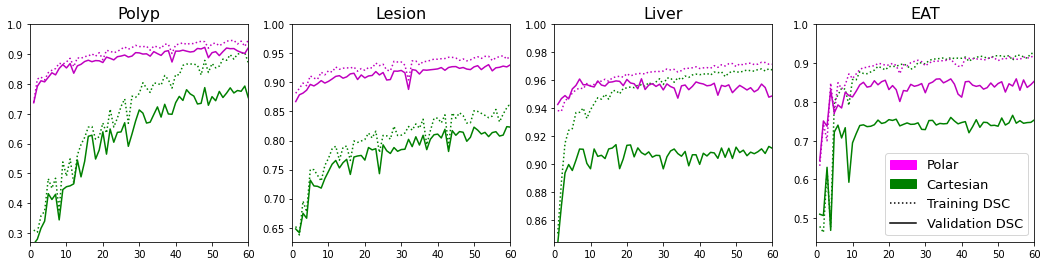
\includegraphics[width=\linewidth]{images/4/training-graphs}
		\caption{The training and validation Dice coefficient (DSC) of the polar and Cartesian U-Net models during training.}
		\label{fig:training}
	\end{figure*}

	\begin{figure}[h]
		\centering
		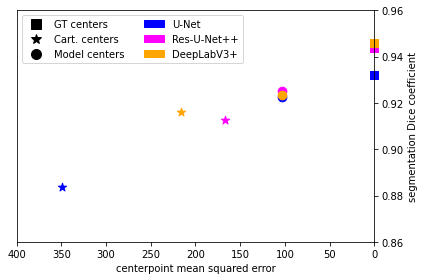
\includegraphics[width=0.65\linewidth]{images/4/mse-vs-dice}
		\caption{The relationship between mean squared errors of the centers used for the polar transformation and segmentation performance of the polar network on the lesion dataset. The mean squared errors are calculated compared to the ground-truth centers.}
		\label{fig:centers-vs-performance}
	\end{figure}
	
We also train several models with both polar and Cartesian coordinates on subsets of the training dataset. Namely, we trained models on 25\%, 50\%, 75\%, and 100\% of the lesion training dataset for 50 epochs. The results of this training are shown in \figref{fig:dataset-vs-dsc}. The polar network is much more data efficient and achieves better results than the cartesian network even with only 25\% of the data.

		\begin{figure}[h]
		\centering
		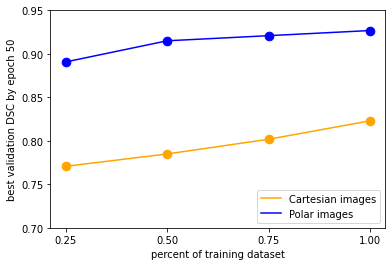
\includegraphics[width=0.65\linewidth]{images/4/dsc-vs-dataset-percent}
		\caption{The best Dice coefficient by epoch 50 for models trained on subsets of the lesion training dataset.}
		\label{fig:dataset-vs-dsc}
	\end{figure}
	
	\section{Discussion}
	
We obtain state-of-the-art results for polyp and lesion segmentation by training common biomedical image segmentation models. In the liver dataset, we achieve state-of-the-art results when compared to other 2D methods, but 3D methods 
achieve the same or slightly better results \cite{valanarasuKiUNetOvercompleteConvolutional2020a}. 
The liver dataset is 
by far the largest dataset we evaluated. As such, improvements gained from 
encoding localization information and reducing dimensionality might not be as large as in smaller 
datasets, since the network has enough data to learn these complex structures.
The EAT dataset is one where the task is not to find a single object, but instead, segment multiple smaller 
pockets of tissue around the heart. This task is more challenging for common models like U-Net and 
requires a more complex approach \cite{zhangAutomaticEpicardialFat2020a}. It is possible that combining 
these existing approaches, namely segmenting the pericardium first, with training on polar coordinates 
would lead to an improvement in the state of the art.

	\begin{figure*}
	\subfloat[Polyp predictions]{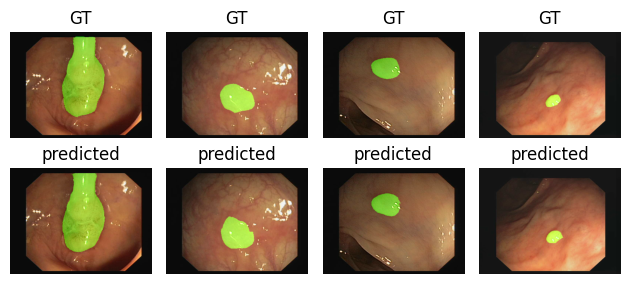
\includegraphics[width=0.49\columnwidth]{images/4/centerpoint_model_output_polyp}}
	\hfill
	\subfloat[Lesion predictions]{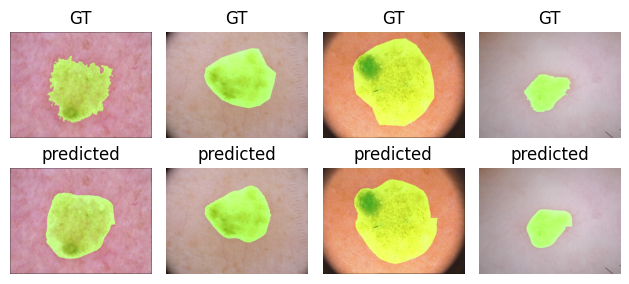
\includegraphics[width=0.49\columnwidth]{images/4/centerpoint_model_output_lesion}} \\
	\subfloat[Liver predictions]{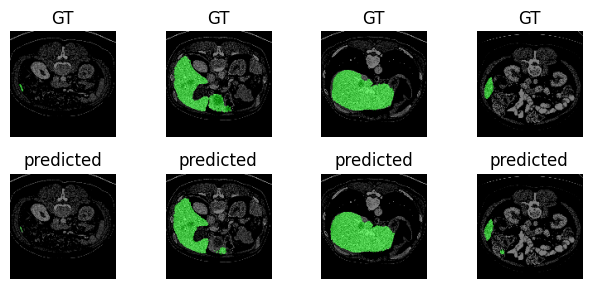
\includegraphics[width=0.49\columnwidth]{images/4/centerpoint_model_output_liver}}
	\hfill
	\subfloat[EAT predictions]{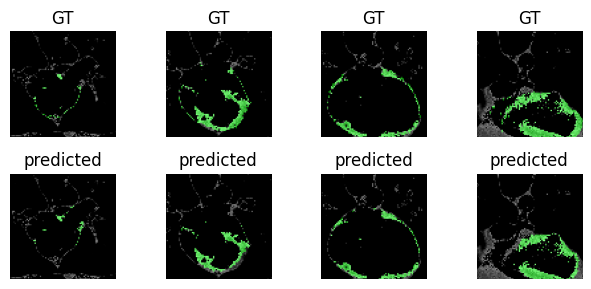
\includegraphics[width=0.49\columnwidth]{images/4/centerpoint_model_output_eat}} \\
	\caption{A random sampling of inverse polar transformed predictions from the polar network with the polar origins predicted from the centerpoint predictor for various datasets. The prediction is shown in green and overlaid on top of the original input image. EAT predictions (d) are cropped and zoomed to better show the predictions.}
	\label{fig:predictions}
	\end{figure*}

We also show that training on polar images leads to a significant improvement in segmentation performance 
when compared to training on Cartesian images for the same network architecture. Additionally, as shown in \figref{fig:training}, the polar 
network portions of our approach converge in much fewer epochs than the Cartesian networks. This is in part due to the location information being encoded in the image 
itself via the polar origin, and in part due to a possible data dimensionality reduction, allowing the 
network to more easily optimize the loss function. The polar networks are also more robust to low dataset 
sample size. This is especially important in biomedical image segmentation where the availability of large 
labeled datasets is often very limited.

Predicting the center point from the Cartesian model, while still an improvement over the plain 
Cartesian network, leads to worse results than those obtained by the center point predictor model. 
We conclude that segmentation is highly dependent on choosing the correct polar origin. This 
dependency is somewhat loosened by adding polar origin augmentation when training the polar 
network.

	\begin{table}[t]
\centering
\def\arraystretch{1.25}
\begin{tabular}{l c c}
 \hline
 Method & DSC & Difference \\ 
 \hline \\ [-2ex]
Cartesian & 0.8315 & - \\
Polar (Cartesian origins) & 0.8918  & +0.0603 \\
Polar (Centerpoint predictor) & 0.9094 & +0.0176  \\
 + centerpoint augmentation & 0.9288 & +0.0194 \\
 + polar network training augmentation & 0.9374 & +0.0086 \\ [1ex]
\hline \\ [-1.5ex]
\end{tabular}
\caption{Ablation study of our approach for the polyp dataset.}
\label{table:ablation}
\end{table}

\figref{fig:predictions} shows a random sampling of predictions from the polar network using the center point predictor for polar origins. Qualitatively, we conclude that the network achieves very good segmentation results, leading to a very high overlap with the target object. The network successfully segments both small and elliptical as well as large and unevenly shaped polyps. On the lesion images, the network predicts a smooth border when sometimes the actual border of the lesion is rough, as shown in the left-most example on \figref{fig:predictions}(b), however, the network still does a good job of delineating a lesion border even when the color of the lesion is very similar to the surrounding skin. The network successfully predicts a liver border both when the liver is very large and very small on the image, showing good scale invariance, but sometimes under segments the liver when multiple connected components are needed. On the EAT dataset, the network successfully learns to segment EAT despite its highly discontinuous and sparse distribution. However, the network sometimes under segments EAT.

Finally, we also perform an ablation study shown in \tabref{table:ablation}. Training on the polar coordinates with the polar origins predicted from the cartesian network yields the largest performance improvement. Predicting the polar origin from the center point predictor as well as adding center point augmentation to the predictor play a roughly equally important role in the performance. Lastly, a small performance improvement is further achieved by using data augmentation when training the polar network.

A potential improvement of our method is to train a single neural network that combines the center-point 
predictor and the segmentation network and is trained end-to-end. In our approach, polar origins are always 
optimized towards the center of mass of the segmented object. Training an end-to-end network would allow 
the polar origins to be optimized for that specific segmentation task. Additionally, the center points could 
be obtained manually from experts, creating a user-guided segmentation approach similar to 
\cite{kimCNNBasedUGS2018}. The center points could also be obtained by a more basic segmentation approach 
like thresholding or other traditional image processing method, leading to a possible reduction in the 
number of required neural network parameters to achieve good segmentation. Furthermore, in our experiments,
we found that the segmentation is dependent on choosing the correct standard deviation of the generated 
heatmaps for training the center point predictor. An improvement to our method could be made by developing
a method to automatically estimate the standard deviation from the training or validation data without needing
to first train the center point predictor.

  \section{Conclusion}
  
  \todo{rewrite this using formulation}
  
We explored training neural networks for biomedical image segmentation on polar transformations on images.
We hypothesized that polar transformations would reduce the dimensionality of the input images, and allow
the network to separately learn localization and fine segmentation of an object.
We showed that training time improves when training on polar images for 
tasks where a single object 
which is roughly elliptical in shape or distribution needs to be segmented. Additionally, we show that training on polar
images achieves state-of-the-art results on small datasets, and achieves near state-of-the-art results on larger
datasets using generic low-parameter-count models like U-Net. We also noted that choosing the correct 
polar origin is essential for improving performance on polar images. Therefore, we proposed two different 
ways of obtaining the polar origin automatically from unlabeled input images. We trained a center-point 
predictor which predicts a heatmap to produce a polar origin, and showed that its performance is better 
than predicting the origin from a segmentation network trained on Cartesian images.
We noted that sometimes our method under segments in examples where multiple objects need to be segmented.

While our approach already produces state-of-the-art results in some cases, our results could be further improved. 
Our approach can be used as a pre-processing step for 
existing and future semantic segmentation methods that use neural networks to provide additional 
segmentation improvement. Therefore, it is possible that our approach could be used in a variety of 
different biomedical and non-medical segmentation applications.







